\section{Introduction}

Galaxies can grow through both internal and external processes. The internal processes include stellar winds, supernova explosion, AGN feedback, secular evolution, and the external processes include mergers and gas accretion. Considering widely accpeted tidal torque theory (TTT), baryons acquire angular momentum from background gravitational tidal field when matter collapses to form a galaxy/halo \citep{1951pca..conf..195H, 1969ApJ...155..393P, 1970Ap......6..320D}, during this process angular momentum conserves, the newly formed stars inherit gaseous dynamical properties \citep{1978MNRAS.183..341W, 1980MNRAS.193..189F, 1998MNRAS.295..319M}. If a galaxy grows only through internal processes, the phenomena of galactic scale gas-star misalignment in velocity fields will not be as popular as we obseved (30$\sim$40\% in elliptical and lenticular galaxies). Thus galaxies with different distributions of velocity fields in gas and stellar components are the ideal laboratory to study the influence of external processes on galaxy evolution, whether they completely reshape the structure of the host galaxies or merely perturb them; whether the strength of influence depends on different physical properties or type of the host galaxies?

The phenomena of misaligned velocity fields between gas and stellar components have been observed ubiquitously in elliptical and lenticular galaxies with a fraction up to 30$\sim$40\% \citep{1992ApJ...401L..79B, 1996MNRAS.283..543K, kannappan_broad_2001, sarzi_sauron_2006, davis_atlas3d_2011, barrera-ballesteros_kinematic_2014, barrera-ballesteros_tracing_2015, chen_growth_2016, jin_sdss-iv_2016}, but much fewer (2$\sim$5\%) in star-forming galaxies \citep{chen_growth_2016, jin_sdss-iv_2016, bryant_sami_2019}. The lower fraction of the galaxies with decoupled gas and star kinematics in gas-rich star forming galaxies is due to that the collision cross-section between pre-existing and accreted gas is large enough to influence the retrograde angular momentum of the accreted gas. The decoupled gas-star kinematics only appears in galaxies where the angular momentum of the accreted gas is larger than the pre-existing gas. While for the gas-poor galaxies with low SFR, the accreted gas would survive for $\sim$1 to 5 Gyr \citep{davis_depletion_2016} since the interaction with existing gas is negligible.

In the last decade, especially since the development of large integral-field spectroscopic surveys, such as CALIFA \citep{2012A&A...538A...8S}, SAMI \citep{2012MNRAS.421..872C} and $\rm ATLAS^{3D}$ \citep{2011MNRAS.413..813C}, series of works have been developed in order to understand the origin of the kinematically misaligned gas components. These studies include morphologies/environments \citep{davis_atlas3d_2011, barrera-ballesteros_kinematic_2014, barrera-ballesteros_tracing_2015, jin_sdss-iv_2016, bassett_formation_2017, 2021MNRAS.505.5075Y}, stellar populations \citep{chen_growth_2016, jin_sdss-iv_2016, bevacqua_sdss-iv_2021}, gas-phase metallicities \citep{chen_growth_2016, jin_sdss-iv_2016}, kinematics \citep{katkov_decoupled_2014, naab_atlas3d_2014, bevacqua_sdss-iv_2021}. Following the development in the observations, gas-star misaligned galaxies are also found in cosmological simulation \citep{osman_strong_2017, bassett_formation_2017, taylor_origin_2018, duckworth_sdss-iv_2019, starkenburg_origin_2019, 2020MNRAS.492.1869D, 2020MNRAS.495.4542D, khoperskov_extreme_2020, khim_stargas_2021}, in which we can trace back the formation histories of the misaligned galaxies, searching for the physical mechanisms responsible for misaligned gas-star kinematics. Although several different mechanisms, such as gas precession and AGN feedback, have been proposed to produce or make it easier to produce misaligned phenomena, all of these works share a common sense that external processes, e.g. merging and gas accretion, play significant roles in the formation of misaligned gas-star components. In particular, \citet{lu_hot_2021} used the IllustrisTNG simulation \citep{marinacci_first_2018, naiman_first_2018, nelson_first_2018, nelson_first_2019, pillepich_first_2018, pillepich_first_2019, springel_first_2018} and found that the gas-star misaligned star-forming disc galaxies have experienced more frequent retrograde mergers (with respect to their stellar spins) throughout their history. During a retrograde merger, gas at the outskirts was first perturbed by the incoming galaxy, becoming misaligned with respect to the existing stellar spin. As gas was then accreted onto the central stellar disk, the galaxy would finally exhibit the gas-star kinematically misaligned feature.

\begin{figure*} 
    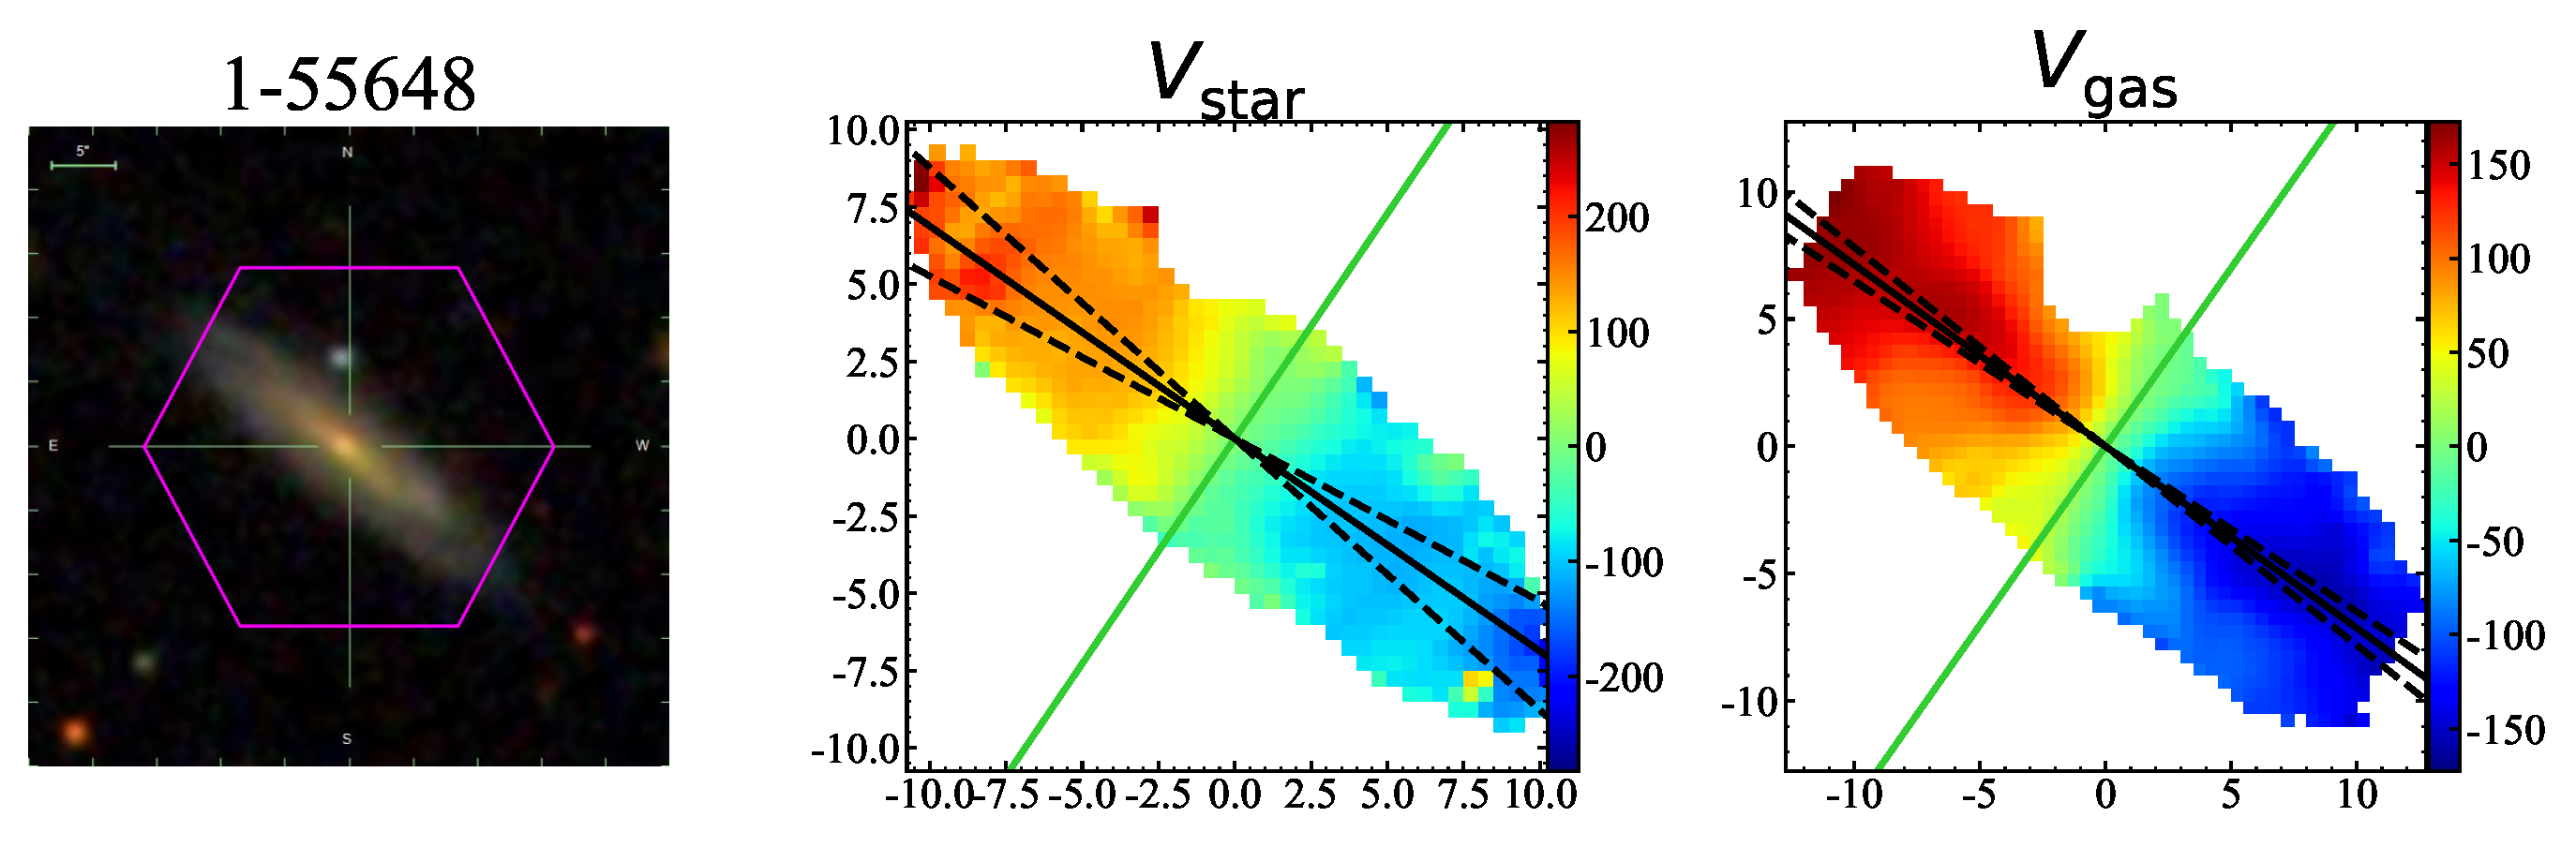
\includegraphics[width=2.0\columnwidth]{pics/explain_PA/PA_1-55648.eps}
    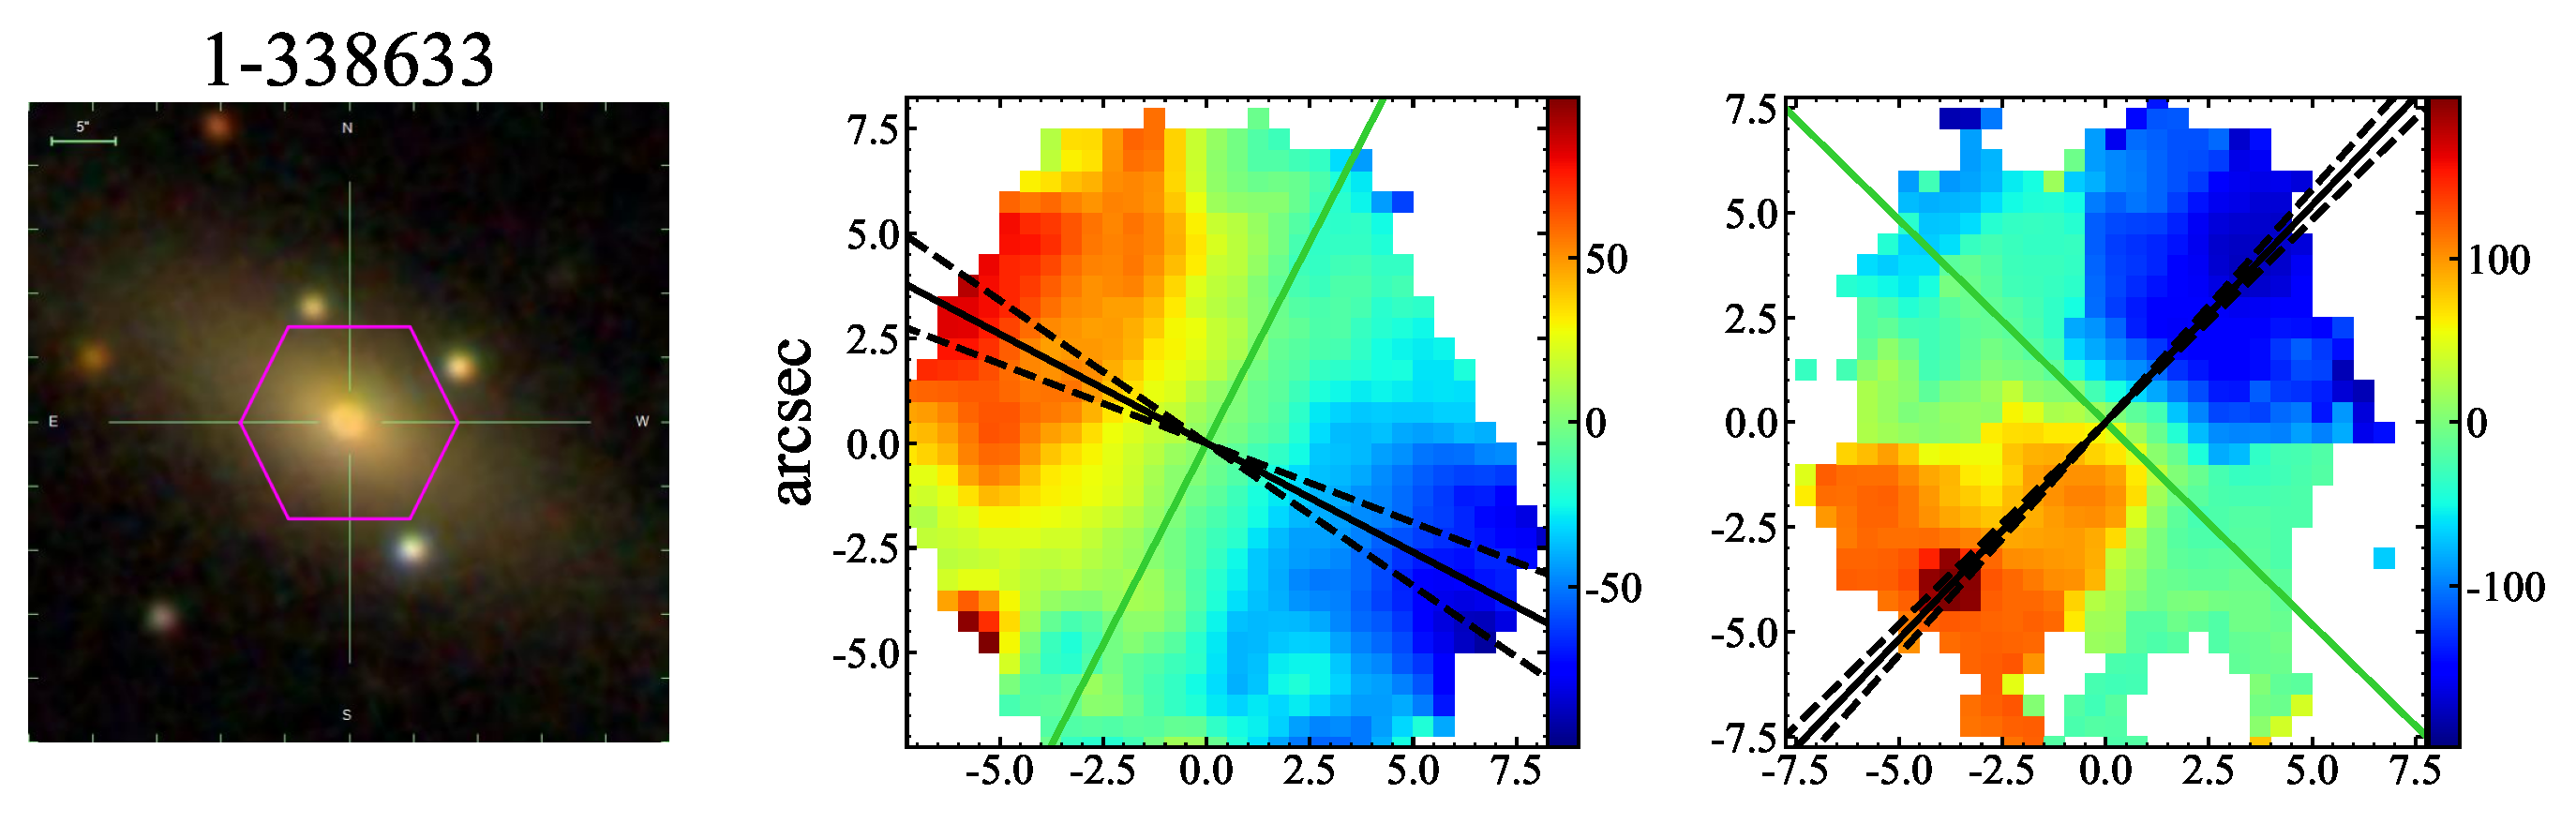
\includegraphics[width=2.0\columnwidth]{pics/explain_PA/PA_1-338633.eps}
    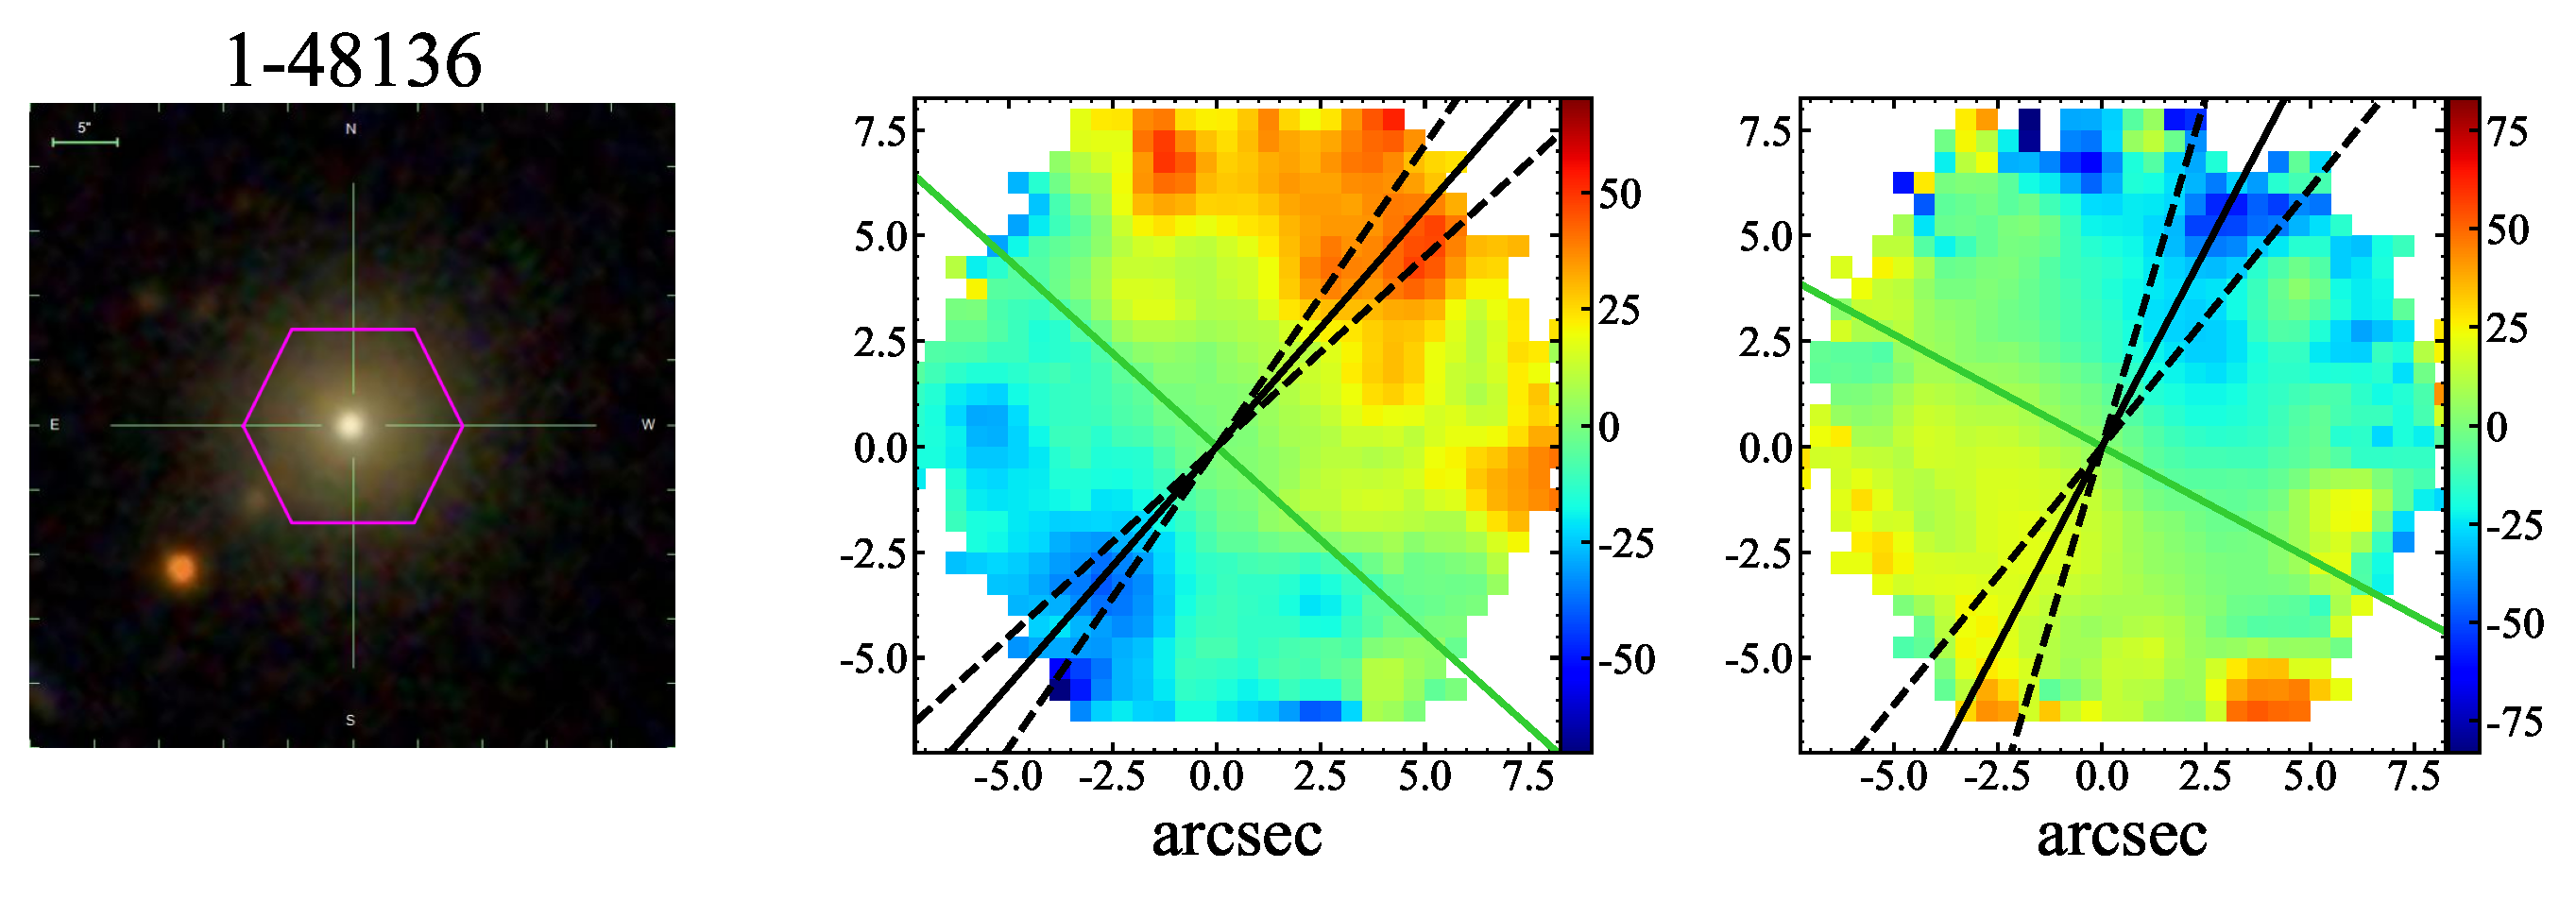
\includegraphics[width=2.0\columnwidth]{pics/explain_PA/PA_1-48136.eps}
    \caption{Examples of three MaNGA galaxies. Each row represents a galaxy (MaNGA ID is shown on the top). The left panel shows the SDSS \textit{g,r,i}-band image, the middle panel shows the stellar velocity field and the right panel shows the gas velocity field. The rotation velocities are indicated by the color bar, the red side is moving away from us while the blue side is approaching us. The solid black lines and green lines in each velocity field show the major and minor axis of the velocity field fitted by Python module FIT\_KINEMATIC\_PA \citep{krajnovic_kinemetry_2006}, while two dashed lines show $\pm 1 \sigma$ error range of PAs. The top row shows a galaxy (MaNGAID 1-55648) that has kinematically aligned stars and gas with $\Delta$PA $= 1^{\circ}$; the middle row shows a galaxy (MaNGAID 1-338633) with gas and stars rotating perpendicularly with $\Delta$PA $= 74^{\circ}$; the bottom row shows a galaxy (MaNGAID 1-48136) with gas and stars counter-rotating with $\Delta$PA $= 167^{\circ}$.}
    \label{fig:explain_PA}
\end{figure*}

In this paper, we select 460 gas-star misaligned galaxies from the internal Product Launch-10 (MPL-10) in Mapping Nearby Galaxies at Apache Point Observatory \citep[MaNGA,][]{2015ApJ...798....7B}, a new internal field spectroscopic survey. As a follow-up work of \cite{jin_sdss-iv_2016}, the sample size is enlarged by a factor of 7. Based on this largest misaligned sample so far, we look into the properties (i.e. kinematics, stellar populations, star formation activities, gas-phase metallicities) of these misaligned galaxies. The paper is organized as follows, In Section \ref{sec:data}, we present the selection of misaligned galaxies and their control samples. In Section \ref{sec:data analysis}, we compare the spatial resolved properties between misaligned galaxies and the control samples. We discuss the observational results in Section \ref{sec:discussion}. In Section \ref{sec:conclusions}, we briefly summarize the results. Throughout this paper, we adopt a flat $\Lambda$CDM cosmology with $\Omega_\Lambda=0.7$, $\Omega_{\rm m}=0.3$, and $H_0=70$ km s$^{-1}$ Mpc$^{-1}$.
